%\PassOptionsToPackage{table}{xcolor}
\documentclass{beamer}
%\usepackage{times,helvet}
%\usepackage{palatino}
\usepackage{epsfig,color}
\usepackage{graphicx}
\usepackage{multirow}
\usepackage{comment}
\usepackage{xspace}
\usepackage{hyperref}
%\PassOptionsToPackage{usenames}{xcolor}
\usepackage{overpic}
\definecolor{lightblue}{rgb}{0.145,0.6666,1}
    \newcommand{\colouredcircle}{%
       \hspace{1em}\tikz{\useasboundingbox (-0.2em,-0.32em) rectangle(0.2em,0.32em); \draw[draw=black,fill=lightblue,line width=0.03em] (0,0) circle(0.18em);}\hspace{1em}}
 \newcommand{\IMPATH}{../../../../htdocs/tutorial/EIDORS_basics}
%\newcommand{\IMPATH}{./}
\mode<presentation>
{
	\usetheme{default} % I sometimes also use Warsaw
	\setbeamertemplate{itemize items}[circle]
	\setbeamertemplate{navigation symbols}{}
}
\setbeamertemplate{footline}
{
  \leavevmode%
  \hbox{%
  \begin{beamercolorbox}[wd=.3\paperwidth,ht=2.25ex,dp=1ex,left]{?}%
\hspace{1mm}
% \includegraphics[width=0.15\paperwidth]
%    {../../../current-docs/CarletonWide_K_186.png}
  \end{beamercolorbox}%
  \begin{beamercolorbox}[wd=.45\paperwidth,ht=2.25ex,dp=1ex,center]{t}%
{\em Conductivity Perturbations}, Adler, Lionheart, 2015/06/03
  \end{beamercolorbox}%
  \begin{beamercolorbox}[wd=.24\paperwidth,ht=2.25ex,dp=1ex,right]{title in head/foot}%
    \insertframenumber{}~/~\inserttotalframenumber\hspace*{1ex}
  \end{beamercolorbox}}%
  \vskip0pt%
}


\usepackage{tikz}
\pgfdeclarelayer{foreground}
 \pgfdeclarelayer{background}
 \pgfsetlayers{background,main,foreground}

\begin{document}


\title[Conductvity Perturbations]{
\vspace{10mm}
~\\
\Huge
{\em
Conductivity Perturbations \\ in EIT
}
\\
\vspace{10mm}
}
\author{
   Andy Adler$^1$ and
   Bill Lionheart$^2$
}
\institute[]{
$^1$Systems and Computer Engineering, Carleton University, Ottawa, Canada
\\
$^2$School of Mathematics, University of Manchester, UK
}
\date{}

\frame{\titlepage} 

\frame{\frametitle{%
EIT Sensitivity \ldots
}
What is sensitivity?
}

\frame{\frametitle{%
EIT Sensitivity \ldots
}
EIT forward problem
\begin{equation*}
   v = F(\sigma)
\end{equation*}
If we are doing
\\ \colouredcircle {\em difference imaging}, 
\\ \colouredcircle analyzing the sensitivity, or
\\ \colouredcircle designing drive and measurement strategies
\\
we want to
know the difference signal.
\begin{equation*}
   \Delta v = F(\sigma + \Delta \sigma) - F(\sigma)
\end{equation*}
 in a homogeneous ($\sigma_h$) medium,
we want the sensitivity to perturbation
for $\Delta \sigma$ in a ROI
\begin{equation*}
   \| \Delta v \| = F(\sigma_h + \Delta \sigma) - F(\sigma_h)
\end{equation*}

}



\frame{\frametitle{%
Two kinds of sensitivity!}

Back in 1986 the first EIT meeting in Sheffield (Physiol Meas 1987 Suppl A)

\fbox{%
\includegraphics[width=.35\columnwidth]{Jossinet-1987.jpg}}%
\fbox{%
\includegraphics[scale=0.3]{BreckonPidcock-1987.jpg}}

\begin{itemize}
\item[\colouredcircle]
Jossinet and  Kardous (pp33--37) showed an experimental
determination of sensitivity using a ball and micro-manipulator
while Seagar, Barber and Brown (pp13--31) gave the formulae for a
offset circular
anomaly 

\item[\colouredcircle]
Breckon and Pidcock (pp77--84) exhibited the Fr\'echet derivative
formula. This is an `infinitesimal' change, is limit as $\Delta
\sigma$ tends to zero.
\end{itemize}

}

\frame{\frametitle{%
Sensitivity in 2D
}
Circular ball and the perturbation of streamlines
\\
\colouredcircle
Contrast $1+ \frac{\Delta \sigma}{\sigma_h}$

\centering
\vspace{3mm}
\begin{tabular}{@{}c@{}c@{}c@{}c@{}c@{}c@{}c@{}}
  $10^{-3}$
& $10^{-2}$
& $10^{-1}$
& $10^{ 0}= 1$
& $10^{ 1}$
& $10^{ 2}$
& $10^{ 3}$
\\
 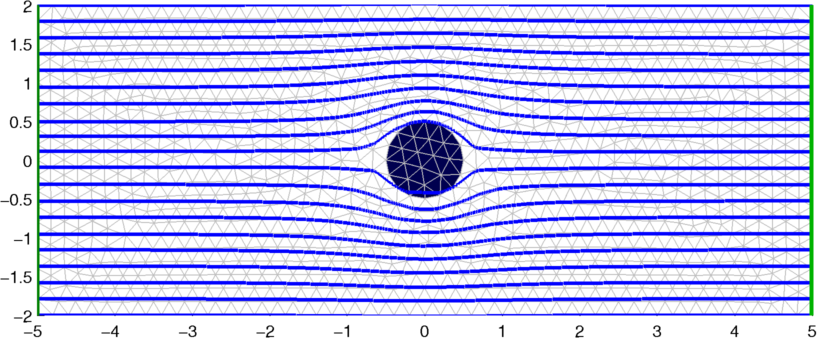
\includegraphics[width=.35\columnwidth, angle=90]
     {\IMPATH/contrasts_04i.png}
&
 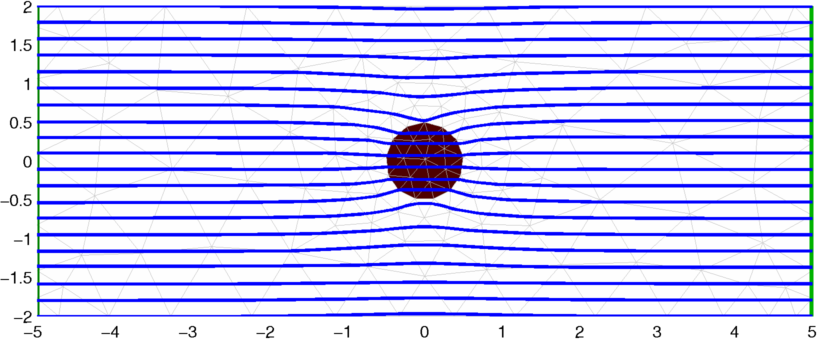
\includegraphics[width=.35\columnwidth, angle=90]
     {\IMPATH/contrasts_04j.png}
&
 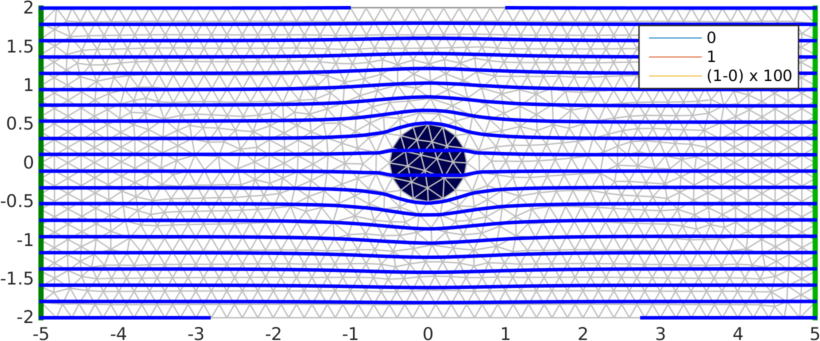
\includegraphics[width=.35\columnwidth, angle=90]
     {\IMPATH/contrasts_04k.png}
&
 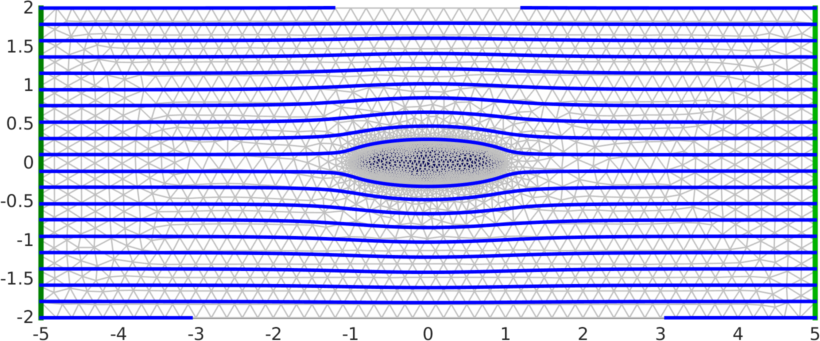
\includegraphics[width=.35\columnwidth, angle=90]
     {\IMPATH/contrasts_04l.png}
&
 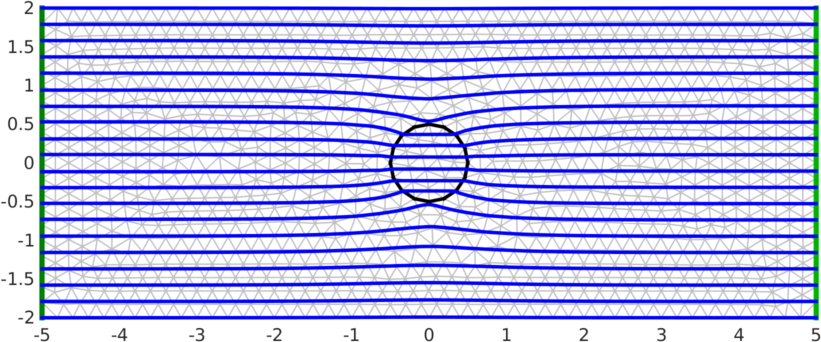
\includegraphics[width=.35\columnwidth, angle=90]
     {\IMPATH/contrasts_04m.png}
&
 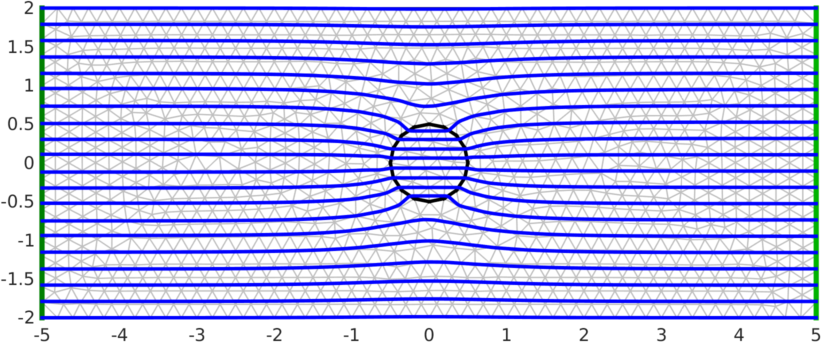
\includegraphics[width=.35\columnwidth, angle=90]
     {\IMPATH/contrasts_04n.png}
&
 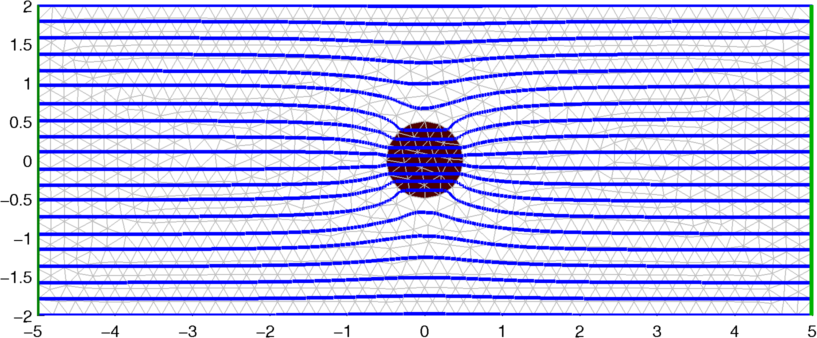
\includegraphics[width=.35\columnwidth, angle=90]
     {\IMPATH/contrasts_04o.png}
\\
 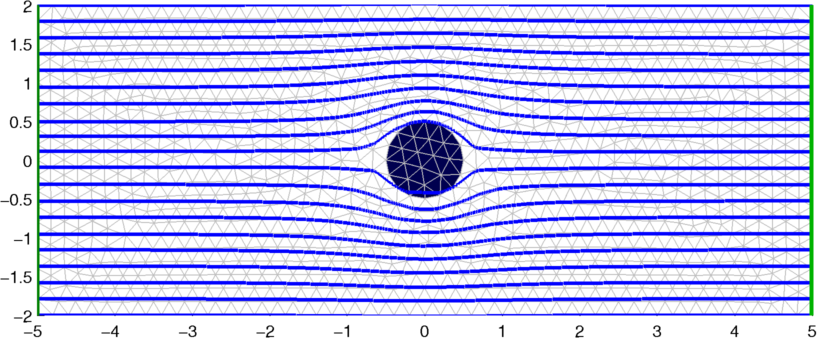
\includegraphics[width=.15\columnwidth, angle=90,trim=330 90 300 80,clip]
     {\IMPATH/contrasts_04i.png}
&
 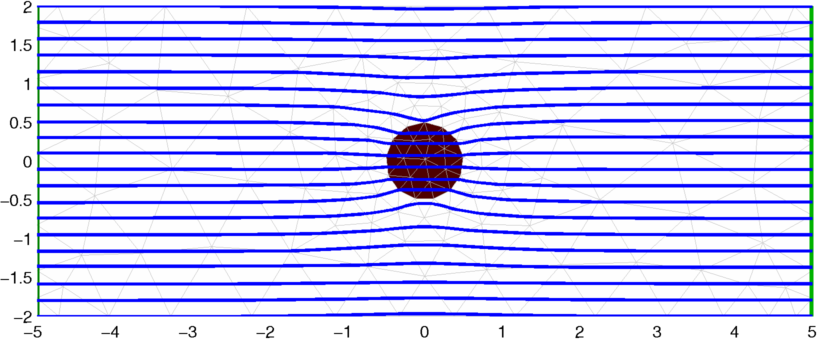
\includegraphics[width=.15\columnwidth, angle=90,trim=330 90 300 80,clip]
     {\IMPATH/contrasts_04j.png}
&
 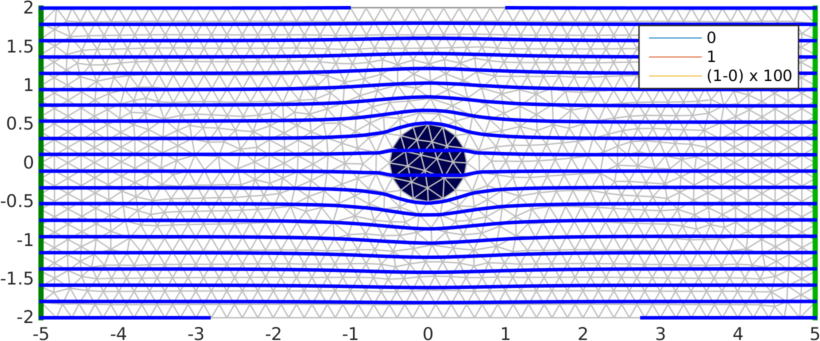
\includegraphics[width=.15\columnwidth, angle=90,trim=330 90 300 80,clip]
     {\IMPATH/contrasts_04k.png}
&
 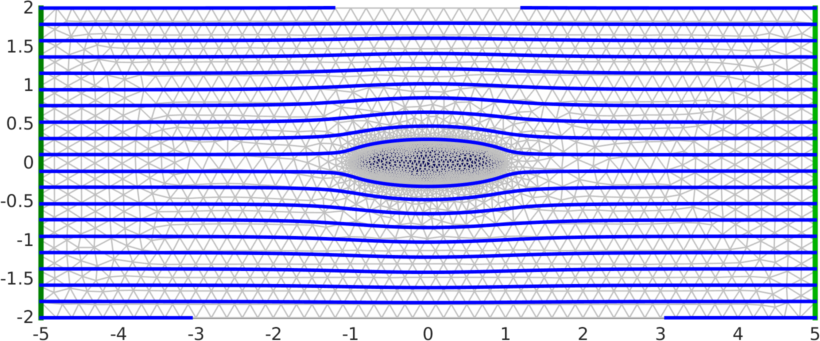
\includegraphics[width=.15\columnwidth, angle=90,trim=330 90 300 80,clip]
     {\IMPATH/contrasts_04l.png}
&
 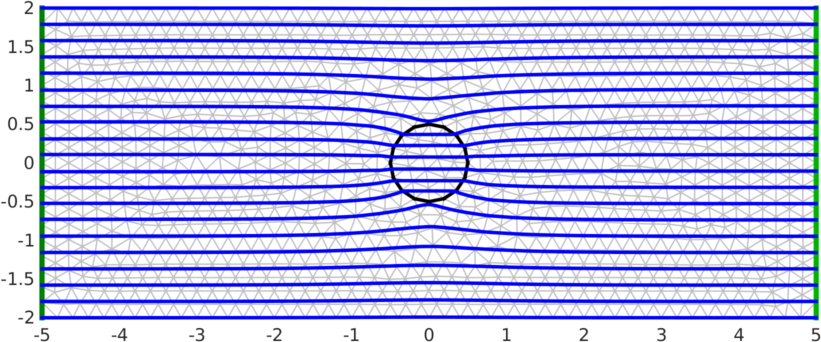
\includegraphics[width=.15\columnwidth, angle=90,trim=330 90 300 80,clip]
     {\IMPATH/contrasts_04m.png}
&
 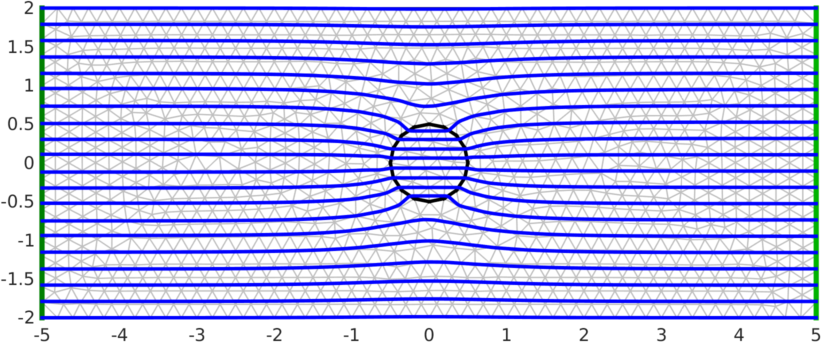
\includegraphics[width=.15\columnwidth, angle=90,trim=330 90 300 80,clip]
     {\IMPATH/contrasts_04n.png}
&
 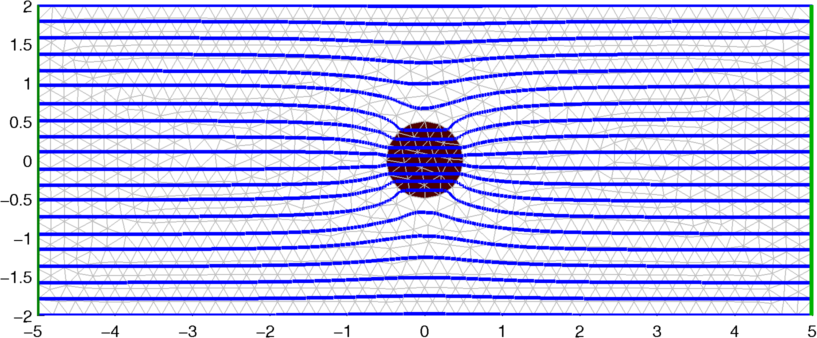
\includegraphics[width=.15\columnwidth, angle=90,trim=330 90 300 80,clip]
     {\IMPATH/contrasts_04o.png}
\end{tabular}
}


\frame{\frametitle{%
Sensitivity in 2D \ldots
}

For a circle in 2D, 
\begin{equation*}
{\rm Signal:~}
\|\Delta v\| \propto \frac{\sigma_h - \Delta \sigma}
                          {\sigma_h + \Delta \sigma}
\end{equation*}

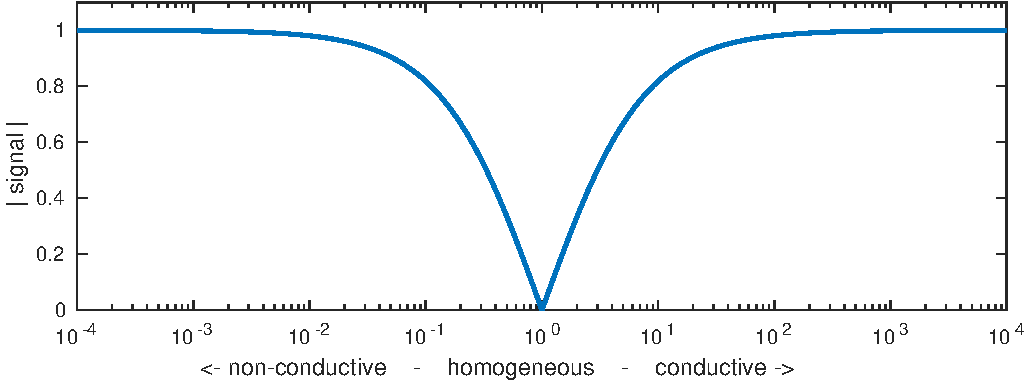
\includegraphics[width=\columnwidth]{two_d_circ_sens.pdf}

So, non-conductive contrasts are as easy to see as conductive ones?
}

\frame{\frametitle{%
Sensitivity in 2D: Non-circular shapes
}

\centering
\vspace{3mm}
\begin{tabular}{@{}c@{}c@{}c@{}c@{}c@{}c@{}c@{}}
  $10^{-3}$
& $10^{-2}$
& $10^{-1}$
& $10^{ 0}= 1$
& $10^{ 1}$
& $10^{ 2}$
& $10^{ 3}$
\\
 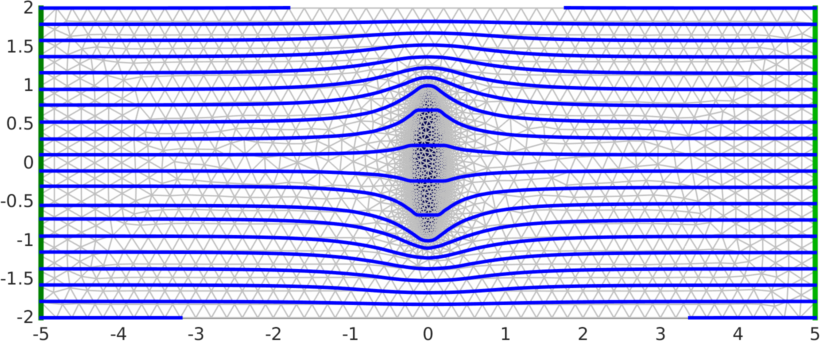
\includegraphics[width=.19\columnwidth, angle=90,trim=290 70 260 60,clip]
     {\IMPATH/contrasts_04b.png}
&
 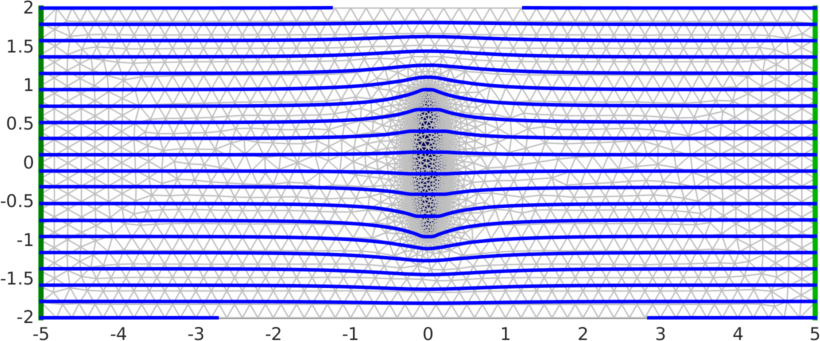
\includegraphics[width=.19\columnwidth, angle=90,trim=290 70 260 60,clip]
     {\IMPATH/contrasts_04c.png}
&
 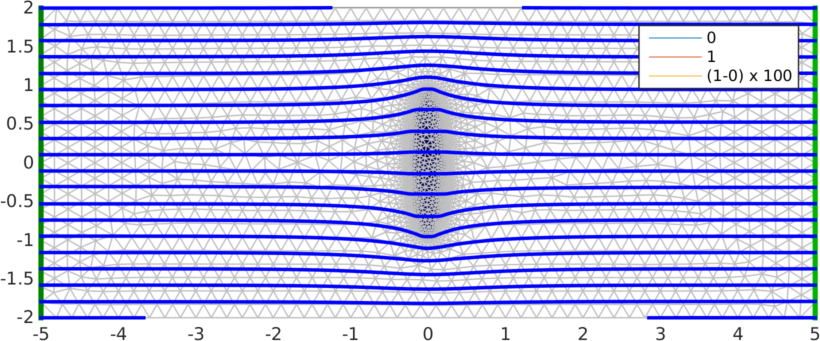
\includegraphics[width=.19\columnwidth, angle=90,trim=290 70 260 60,clip]
     {\IMPATH/contrasts_04d.png}
&
 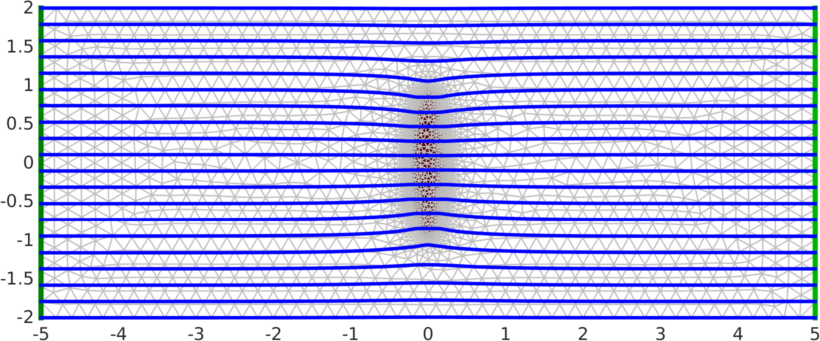
\includegraphics[width=.19\columnwidth, angle=90,trim=290 70 260 60,clip]
     {\IMPATH/contrasts_04e.png}
&
 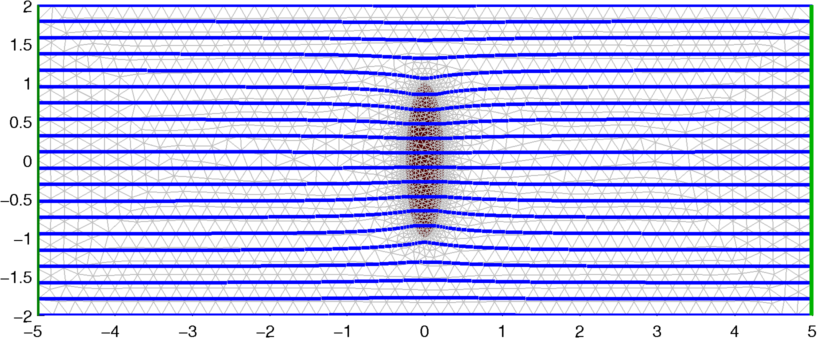
\includegraphics[width=.19\columnwidth, angle=90,trim=290 70 260 60,clip]
     {\IMPATH/contrasts_04f.png}
&
 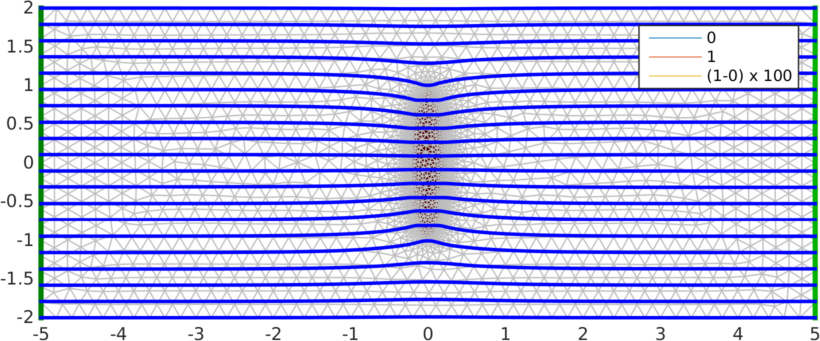
\includegraphics[width=.19\columnwidth, angle=90,trim=290 70 260 60,clip]
     {\IMPATH/contrasts_04g.png}
&
 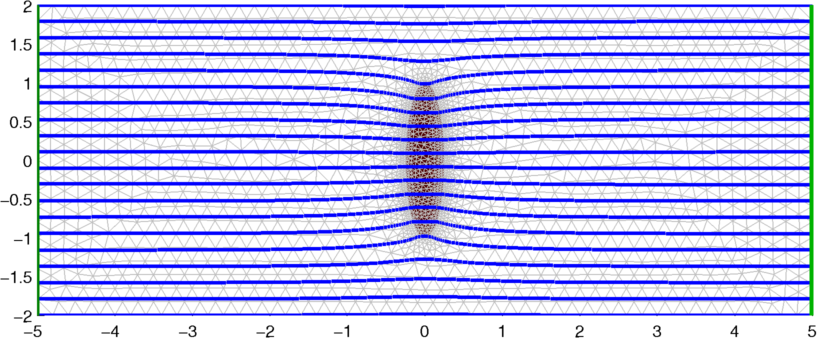
\includegraphics[width=.19\columnwidth, angle=90,trim=290 70 260 60,clip]
     {\IMPATH/contrasts_04h.png}
%
%
%
\\
 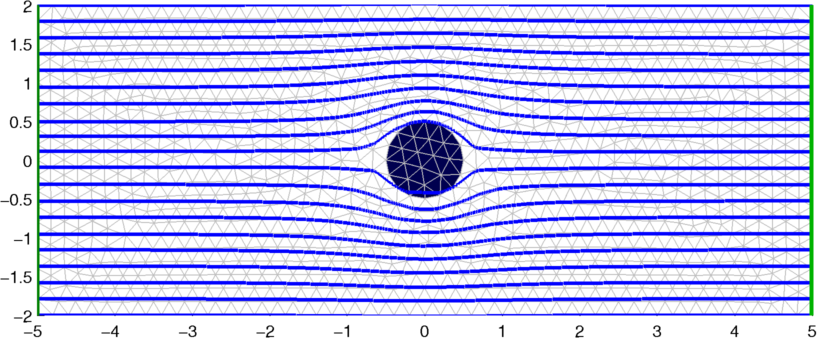
\includegraphics[width=.19\columnwidth, angle=90,trim=290 70 260 60,clip]
     {\IMPATH/contrasts_04i.png}
&
 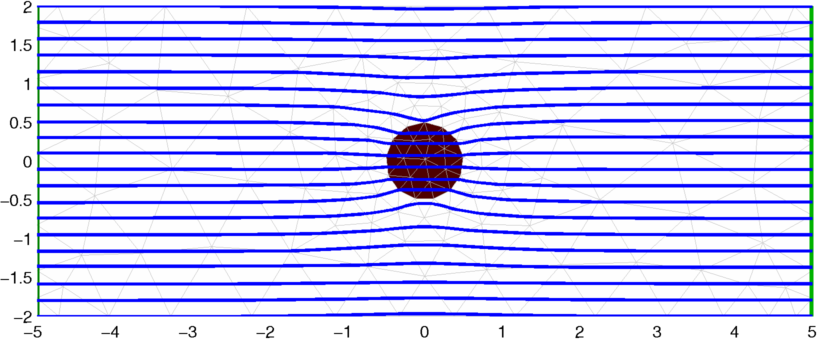
\includegraphics[width=.19\columnwidth, angle=90,trim=290 70 260 60,clip]
     {\IMPATH/contrasts_04j.png}
&
 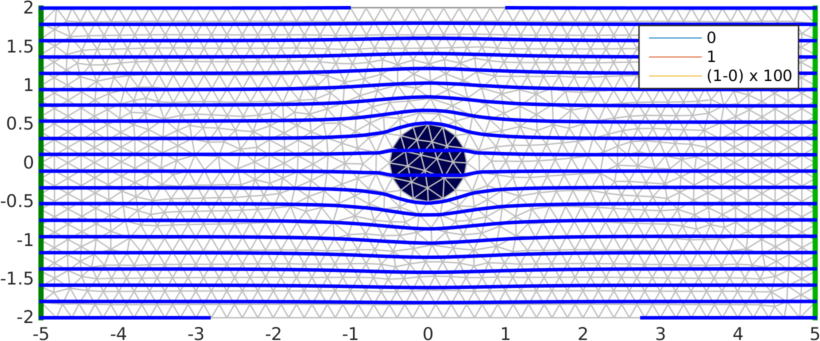
\includegraphics[width=.19\columnwidth, angle=90,trim=290 70 260 60,clip]
     {\IMPATH/contrasts_04k.png}
&
 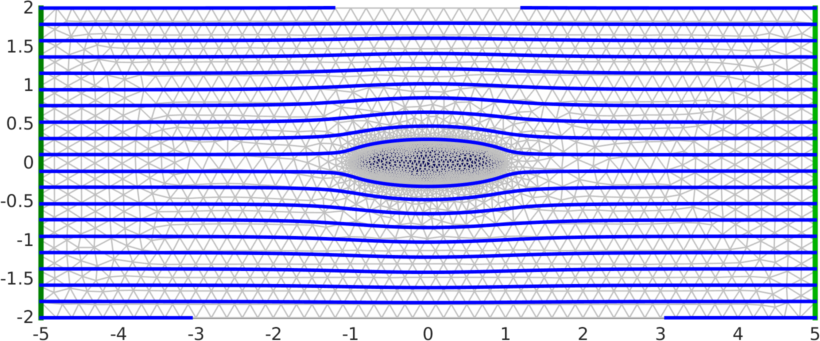
\includegraphics[width=.19\columnwidth, angle=90,trim=290 70 260 60,clip]
     {\IMPATH/contrasts_04l.png}
&
 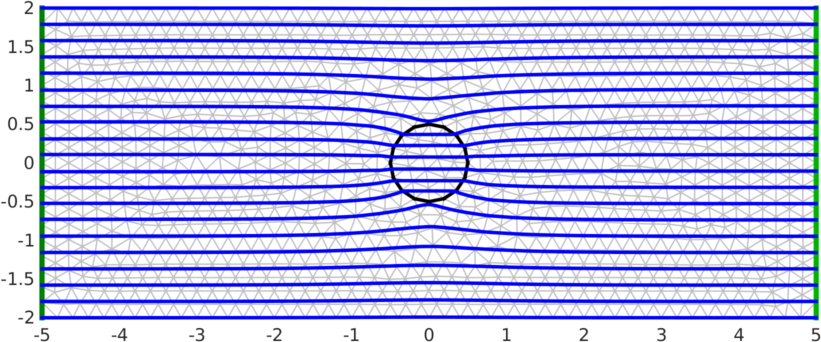
\includegraphics[width=.19\columnwidth, angle=90,trim=290 70 260 60,clip]
     {\IMPATH/contrasts_04m.png}
&
 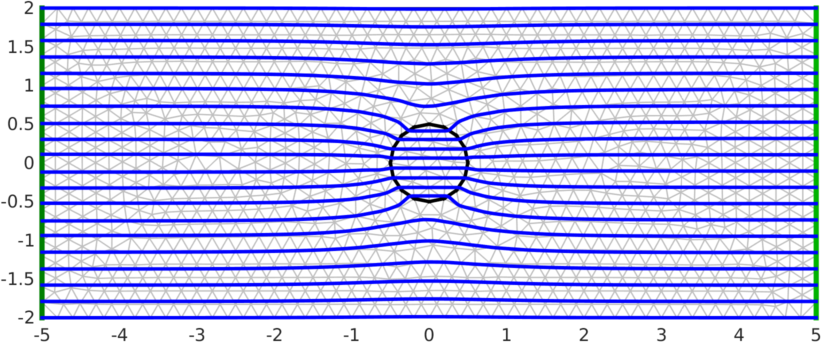
\includegraphics[width=.19\columnwidth, angle=90,trim=290 70 260 60,clip]
     {\IMPATH/contrasts_04n.png}
&
 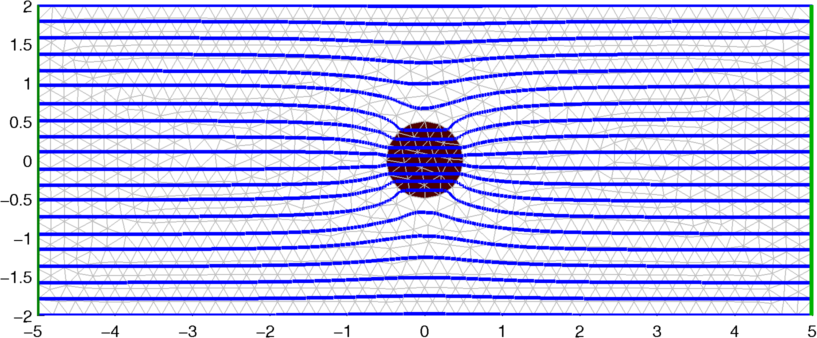
\includegraphics[width=.19\columnwidth, angle=90,trim=290 70 260 60,clip]
     {\IMPATH/contrasts_04o.png}
%
%
%
\\
 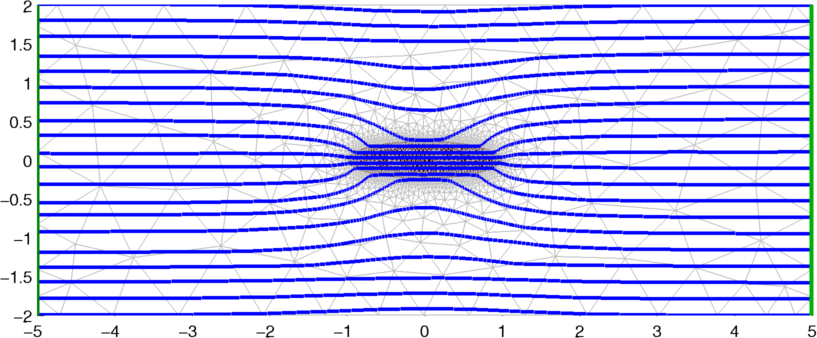
\includegraphics[width=.19\columnwidth, angle=90,trim=290 70 260 60,clip]
     {\IMPATH/contrasts_04p.png}
&
 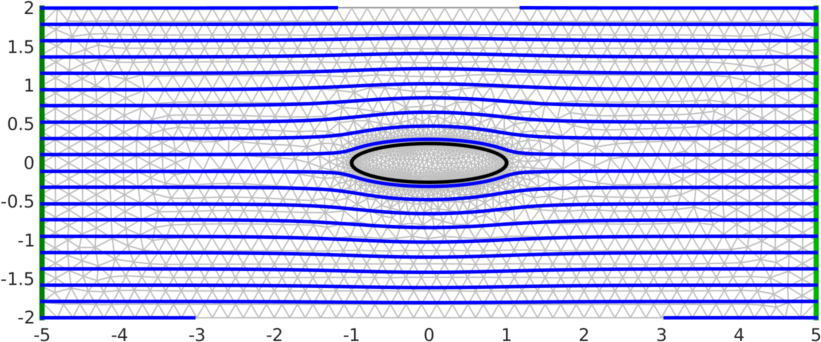
\includegraphics[width=.19\columnwidth, angle=90,trim=290 70 260 60,clip]
     {\IMPATH/contrasts_04q.png}
&
 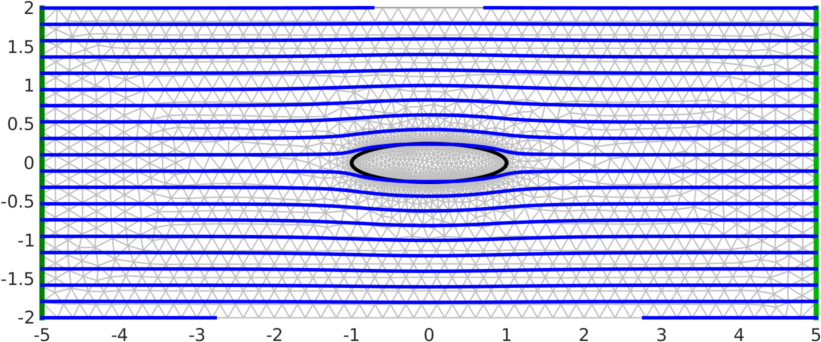
\includegraphics[width=.19\columnwidth, angle=90,trim=290 70 260 60,clip]
     {\IMPATH/contrasts_04r.png}
&
 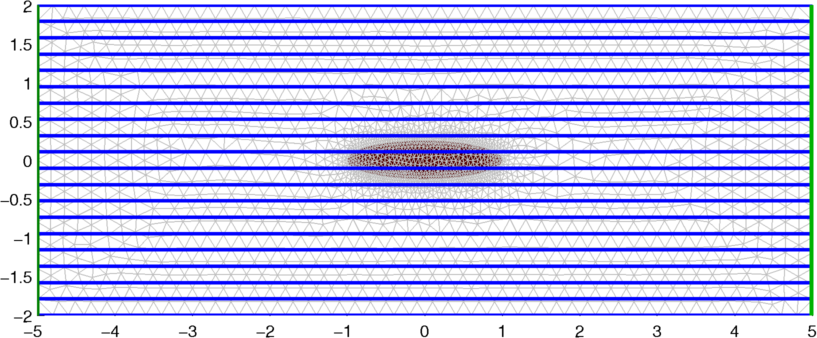
\includegraphics[width=.19\columnwidth, angle=90,trim=290 70 260 60,clip]
     {\IMPATH/contrasts_04s.png}
&
 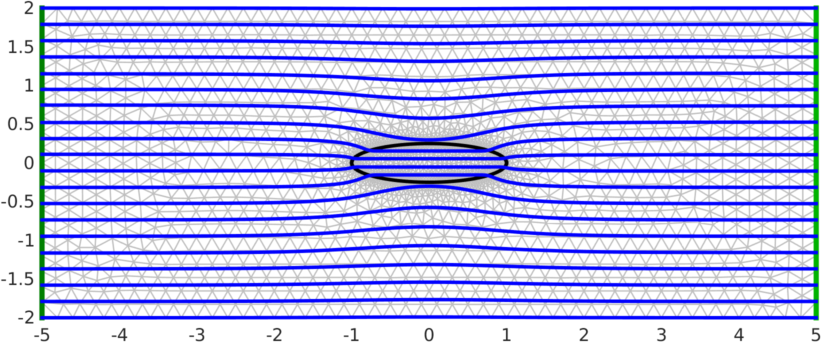
\includegraphics[width=.19\columnwidth, angle=90,trim=290 70 260 60,clip]
     {\IMPATH/contrasts_04t.png}
&
 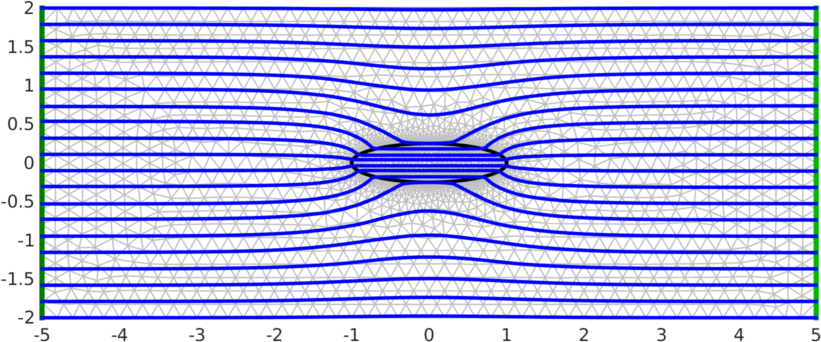
\includegraphics[width=.19\columnwidth, angle=90,trim=290 70 260 60,clip]
     {\IMPATH/contrasts_04u.png}
&
 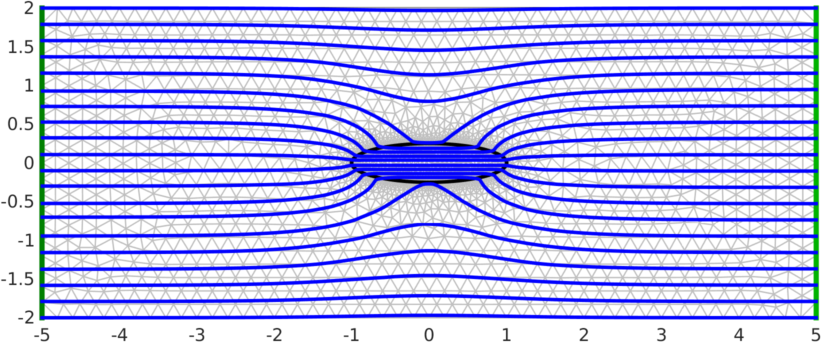
\includegraphics[width=.19\columnwidth, angle=90,trim=290 70 260 60,clip]
     {\IMPATH/contrasts_04v.png}
\end{tabular}
}


\frame{\frametitle{%
Sensitivity \ldots
}
We see that

\colouredcircle
Non-conductive object most visible when 
{\em against the streamlines}

\colouredcircle
Conductive object most visible when 
{\em with the streamlines}

~\\
But in 3D EIT, there are two directions with, and one against.
\begin{center}
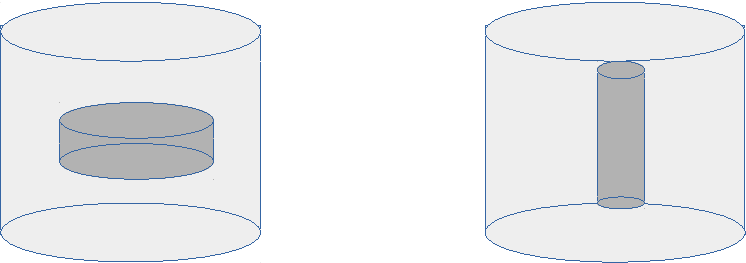
\includegraphics[width=0.7\columnwidth]{diagram.pdf}
\\
\hspace{3mm} Conductive \hspace{25mm} Non-conductive
\end{center}
}

\frame{\frametitle{%
Sensitivity in 3D
}
\begin{center}
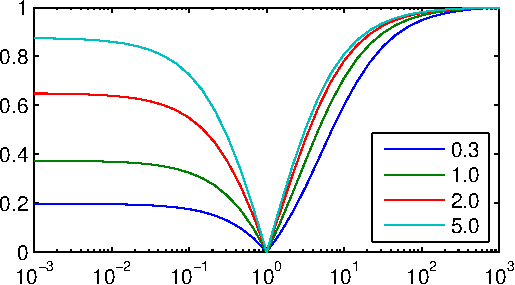
\includegraphics[width=\columnwidth]{signal.pdf}
\\
Normalized signal vs. conductivity contrast, for 
different ratios of height to radius of ROI.
\end{center}
}

\frame{\frametitle{%
Polarization tensor
}

\colouredcircle The so called polarization or polarizability tensor of  P\'olya and Szeg\"o
gives an expression for the dipole moment of the perturbation in potential due to an object with a finite conductivity contrast.
\\
\colouredcircle For an ellipsoid there is an explicit formula that includes the {\em saturation} so it is better than than the linear approximation in this respect
\\
\colouredcircle It is a good approximation for well separated objects distant from the boundary, independent of boundary shape.


}


\frame{\frametitle{%
What does direction sensitivity tell us?
}

\begin{itemize}
\item[\colouredcircle]
Reconstruction algorithms have been based on 
 linear sensitivity. Should we use non-linear 
 sensitivites?

\item[\colouredcircle]
Conductive contrast agents can be seen; no-one has
  ever succeeded with non-conductive contrasts. 
  Does this explain why?
\end{itemize}
}

\end{document}

